\begin{figure}[htbp]
    \centering
    \begin{minipage}{0.48\textwidth}
        \centering
        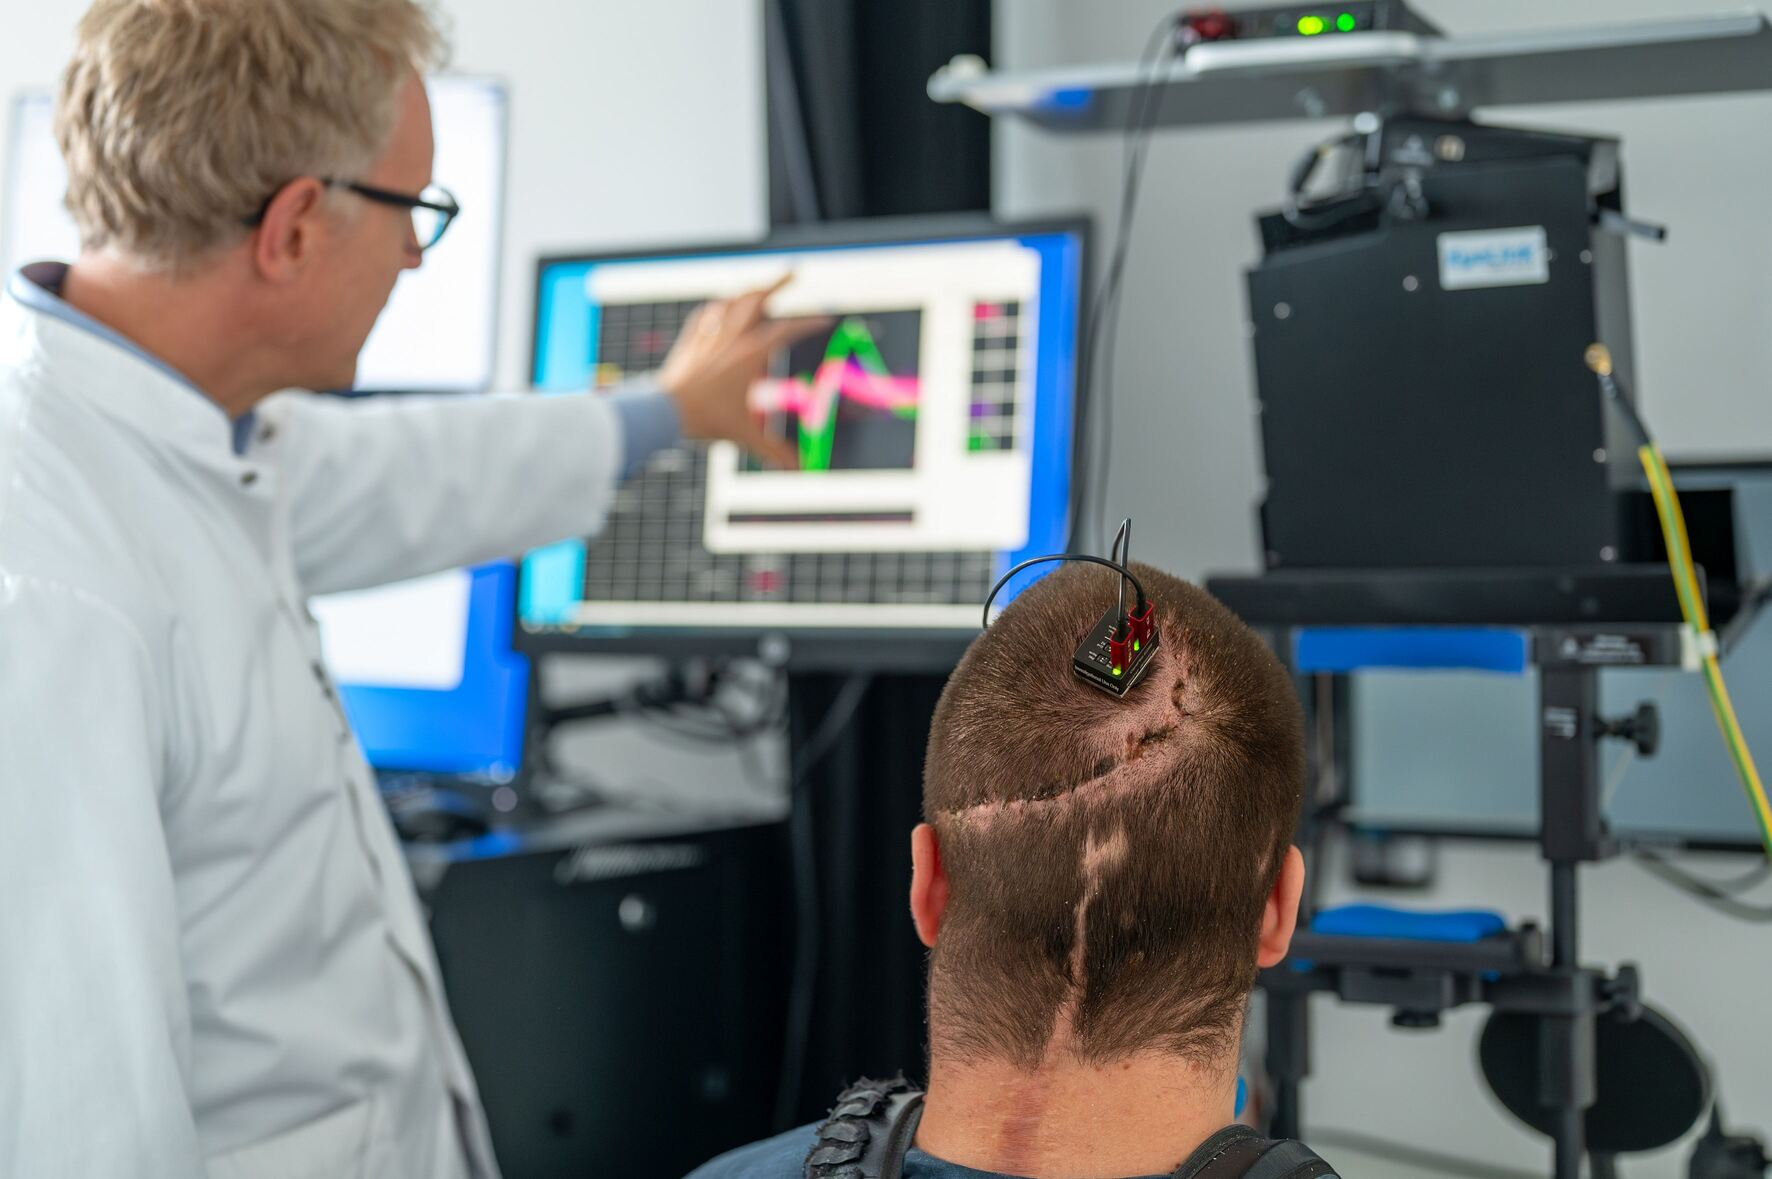
\includegraphics[width=\linewidth]{imagenes/ecog.jpg}
    \end{minipage}
    \hfill
    \begin{minipage}{0.48\textwidth}
        \centering
        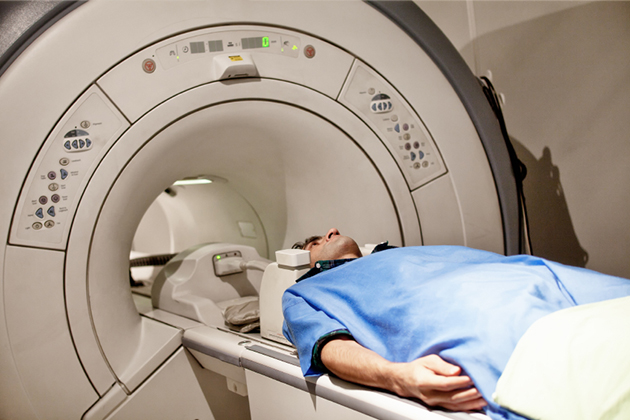
\includegraphics[width=\linewidth]{imagenes/fmri.jpg}
    \end{minipage}
    \caption[Ejemplos de adquisición invasiva y no invasiva]{Ejemplos de adquisición invasiva y no invasiva. A la izquierda, un registro ECoG ilustra la proximidad de los electrodos a la corteza. A la derecha, la fMRI muestra una alternativa no invasiva. \newline Fuentes: izquierda, Kathrin Czoppelt / TUM Klinikum; derecha, Cadena SER Cantabria, \protect\url{https://cadenaser.com/cantabria/2023/05/06/el-hospital-de-laredo-contara-con-una-resonancia-magnetica-ser-castro-urdiales/}.}
    \label{fig:ecog_fmri}
\end{figure}
